\documentclass[aps,prd,10pt,nofootinbib,twocolumn,superscriptaddress,floatfix,notitlepage]{revtex4-1}

\usepackage{graphicx}
\usepackage{amsmath,amsfonts,amssymb}
\usepackage{color}
\usepackage[breaklinks,colorlinks,urlcolor=blue,citecolor=blue,linkcolor=magenta]{hyperref}
\usepackage{verbatim}
\usepackage{enumitem}
\usepackage{aas_macros}

\usepackage{tikz}

\newcommand{\Msun}{M_\odot}
\newcommand{\td}{{\rm d}}
\newcommand{\vect}[1]{\boldsymbol{#1}}
\DeclareMathOperator{\artanh}{artanh}
\DeclareMathOperator{\arcoth}{arcoth}

\newcommand{\be}{\begin{equation}}
\newcommand{\ee}{\end{equation}}
\newcommand{\bea}{\begin{equation} \begin{aligned}}
\newcommand{\eea}{\end{aligned} \end{equation}}
\newcommand{\Gala}[1]{{\color{orange} (#1 -- Gala)}}

\def\lsim{\mathrel{\raise.3ex\hbox{$<$\kern-.75em\lower1ex\hbox{$\sim$}}}}
\def\gsim{\mathrel{\raise.3ex\hbox{$>$\kern-.75em\lower1ex\hbox{$\sim$}}}}

\newcommand{\R}[1]{{\color{red} #1}}
\newcommand{\B}[1]{{\color{blue} #1}}


\begin{document}

\title{Learning weak lensing magnifications}

\author{Galymzhan Baltabay}
\email{galymzhan.baltabay@kbfi.ee}
\affiliation{Laboratory of High Energy and Computational Physics, KBFI, R{\"a}vala 10, Tallinn, 10143, Estonia}
\affiliation{Department of Cybernetics, Tallinn University of Technology, Akadeemia tee 21, 12618 Tallinn, Estonia}

\author{Ville Vaskonen}
\email{ville.vaskonen@kbfi.ee}
\affiliation{Laboratory of High Energy and Computational Physics, KBFI, R{\"a}vala 10, Tallinn, 10143, Estonia}

\begin{abstract}
Gravitational-wave standard sirens provide direct, calibration-free measurements of the luminosity distance, and the scatter that weak lensing by intervening structure induces around the mean Hubble diagram is itself a probe of cosmic structure, complementary to the mean distance-redshift relation~\cite{Vaskonen:2026ubd}. Predicting the resulting magnification probability distribution $dP/d\mu$ accurately, however, requires summing the lensing contribution of a large, stochastically realized population of halos, filaments, and their substructure, a computation too slow to repeat at every point of a cosmological parameter scan. We extend the stochastic lensing model of Ref.~\cite{Vaskonen:2026ubd} by adding the contribution of dark matter subhalos and by replacing its independent (Poisson) halo and filament counts with a correlated treatment of large-scale clustering, and we train a conditional normalizing-flow emulator that reproduces the resulting $dP/d\mu$ as a function of the source redshift and the full six-dimensional set of cosmological parameters $\vect\Theta = \{h,\Omega_M,\Omega_B,\sigma_8,n_s,z_{\rm eq}\}$. The emulator matches the simulator ... \Gala{also we changed the As to sigma8}
\end{abstract}


\maketitle

\section{Introduction}
Gravitational waves (GWs) from compact binary mergers with an identified electromagnetic (EM) counterpart are standard sirens, whose luminosity distance is read directly off the waveform amplitude without a distance-ladder calibration. Ref.~\cite{Vaskonen:2026ubd} showed that the scatter weak gravitational lensing induces around the mean luminosity distance-redshift relation is itself sensitive to the amplitude of matter fluctuations, $\sigma_8$, complementing the standard-siren measurement of the Hubble constant $H_0$ and the matter abundance $\Omega_M$. A population of $\mathcal{O}(100)$ bright sirens from third-generation detectors could reach a competitive measurement of $\sigma_8$ this way.

Exploiting this scatter for cosmological inference requires an accurate model of the magnification probability distribution $dP/d\mu$. One route is ray tracing through the density field of cosmological $N$-body simulations~\cite{Holz:1997ic,Holz:2004xx,Takahashi:2011qd,Takahashi:2017hjr}. To accelerate inference with such simulations, machine-learning emulators such as ACE-Lensing~\cite{Turker:2025rdt} have been trained directly on $N$-body ray-tracing catalogs. However, $N$-body simulations are limited by particle mass resolution, imposing a high halo mass cutoff (per particle mass resolution $\approx 10^{9}\,\Msun$) and smoothing out small-scale substructure. As a result, they fail to populate the high-magnification tail of $dP/d\mu$, which is generated by rare, compact structures close to the line of sight~\cite{DES:2025omh}. The stochastic approach of Refs.~\cite{Kainulainen:2009dw,Kainulainen:2010at,Kainulainen:2011zx}, implemented for bright sirens in Ref.~\cite{Vaskonen:2026ubd}, instead builds $dP/d\mu$ by directly summing the contributions of a Monte Carlo-realized population of discrete lenses down to $10^7\,\Msun$, resolving magnifications that $N$-body ray tracing misses at a fraction of the computational cost. Even so, evaluating $dP/d\mu$ at the many points of a cosmological parameter space required for Markov chain Monte Carlo inference remains expensive, since each evaluation requires a fresh Monte Carlo realization of the lens population. This motivates building a fast, differentiable neural emulator directly for the stochastic lens model.

In this work we extend the stochastic lensing model of Ref.~\cite{Vaskonen:2026ubd} in two ways. First, we add the previously unmodeled contribution of dark matter subhalos, sampling the substructure of every lensing halo down to a fixed mass floor and subtracting the corresponding mass from the smooth halo profile so that the total halo mass is conserved in every realization. Second, we replace the independent Poisson realization of halo and filament counts with a physically motivated treatment of their large-scale clustering, correlating the lens population along the line of sight with a stochastic realization of the underlying density field, together with the sub-threshold background contribution. We then train a conditional normalizing-flow emulator that reproduces the resulting $dP/d\mu$ as a function of the source redshift $z_s$ and the cosmological parameters $\vect\Theta = \{h,\Omega_M,\Omega_B,\sigma_8,n_s,z_{\rm eq}\}$, matching the accuracy of existing emulators while incorporating this extended physical model.

The remainder of this paper is organized as follows. In Sec.~\ref{sec:lensing} we describe the stochastic lensing model, including the clustering of field halos, the subhalo contribution, and the resulting magnification distribution. In Sec.~\ref{sec:ml} we describe the emulator and its training. In Sec.~\ref{sec:comparison} we compare our model and its emulator with earlier work. We conclude in Sec.~\ref{sec:conclusions}.

\B{... ray tracing through universes generated with N-body simulations~\cite{Holz:1997ic,Holz:2004xx,Takahashi:2011qd,Takahashi:2017hjr} ... N-body simulations do not have sufficient resolution to accurately reconstruct the lensing magnification distribution~\cite{DES:2025omh}... stochastic approach~\cite{Kainulainen:2009dw,Kainulainen:2010at,Kainulainen:2011zx} ... machine learning emulator~\cite{Turker:2025rdt} ...}
\Gala{remove blue when you feel its not needed}

\section{Weak lensing}
\label{sec:lensing}
Weak gravitational lensing by structures near the line of sight magnifies the observed signal by a factor $\mu$. Accordingly, the apparent luminosity distance is given by
\be
    D_L(z) = \frac{\tilde{D}_L(z)}{\sqrt{\mu}} \,,
\ee
where $\tilde{D}_L(z)$ denotes the luminosity distance-redshift relation in a homogeneous and isotropic universe. 

In the following we briefly describe the stochastic approach that we use for the computation of the distribution of weak lensing magnifications, focusing on how we extend the lens modeling by including DM subhalos.


\subsection{Stochastic approach}

The lensing magnification is given by
\be \label{eq:mueq}
	\mu = \frac{1}{(1-\kappa)^2 - \gamma^2} \,\B{,}
\ee
where the convergence $\kappa$ and the shear $\gamma = \sqrt{\gamma_1^2+\gamma_2^2}$ are, in the weak-lensing approximation, obtained by summing the contributions of individual lenses: $\kappa = \sum_j \kappa_\epsilon(\vect\theta_j)$, $\gamma_1 = \sum_j \gamma_\epsilon(\vect\theta_j) \cos\phi_j$ and $\gamma_2 = \sum_j \gamma_\epsilon(\vect\theta_j) \sin\phi_j$. Here $\phi_j$ denotes the polar angle of the lens position in the lens plane, defined with respect to a coordinate system common to all lenses, and $\vect\theta_j$ encodes the lens redshift $z_j$, its projected distance $r_j$ from line-of-sight to the source, and parameters describing the lens properties and orientation.

We include lensing contributions from field halos, subhalos, and filaments. The field halos and filaments are modeled as in~\cite{Vaskonen:2026ubd}. The new ingredient included in this study is the contribution of subhalos. Furthermore, we introduce an improved treatment of the clustering of field halos.

\subsubsection{Clustering}

Long-wavelength linear density perturbations modulate the spatial distribution of halos. The resulting change in the halo number density is governed by the halo bias $b(M,z)$, which increases with halo mass $M$ because massive  halos originate from increasingly rare peaks of the primordial density field. 

We estimate the halo clustering using the one-dimensional density field $\delta_{\rm 1D}(z) \equiv \delta_{\rm 1D}(d_c(z))$, obtained by smoothing the three-dimensional density field isotropically with a window of radius $R_{\rm s}$ before projecting onto the line of sight. Its power spectrum is\footnote{This generalizes the pencil-beam construction of Ref.~\cite{1991ApJ...379..482K}, whose $P_{\rm 1D}(k_\parallel)=\int_{k_\parallel}^\infty \td k\,k\,P(k)/(2\pi)$ is recovered in the $R_{\rm s}\to0$ limit.}
\be
    P_{\rm 1D}(k_\parallel) = \frac{1}{2\pi} \int_{k_\parallel}^\infty \!\td k \, k \, P(k) \tilde{W}^2(R_{\rm s} k) \,,
\ee
The smoothing suppresses the contribution of scales smaller than $R_{\rm s}$ both along and perpendicular to the line of sight. We use the real-space top-hat window function and fix $R_s = 20\,$Mpc. We show later how changing $R_s$ impacts our results. 

On a periodic path of length $L$, padded beyond the source distance $d_c(z_s)$ so that the periodicity does not spuriously correlate structure near the observer with that near the source, the 1D density field is given by
\be
    \delta_{\rm 1D}(z) = \frac{1}{L} \sum_{n\geq 1} \tilde\delta_n e^{i k_n d_c(z)} + {\rm c.c.} \,, \quad k_n= \frac{2\pi n}{L} \,,
\ee
where $d_c(z)$ denotes the comoving distance and mode orthogonality gives $\langle\tilde\delta_n\tilde\delta_{n'}^*\rangle=LP_{\rm 1D}(k_n)\delta_{nn'}$. The real and imaginary parts of  $\tilde\delta_n$ are independent Gaussian random variables with equal variance 
\be
    \sigma_n^2 = \frac{L}{2} P_{\rm 1D}(k_n) \,. 
\ee    
Given a realization of the 1D density field $\delta_{\rm 1D}(z)$, the number density of field halos along the line of sight is
\be \label{eq:n}
    \frac{\td n(z)}{\td \ln M} = \lambda(M,z) \frac{\td \bar{n}(z)}{\td \ln M} \,,
\ee
where \footnote{To ensure positivity of $n$ we use the lognormal model of Ref.~\cite{1991MNRAS.248....1C} rather than the linear one, $\lambda(M,z) = 1+\tilde{b}(M,z)\,\delta_{\rm 1D}(z)$.}
\be
    \lambda(M,z) = \exp\!\left[ \tilde{b}(M,z) \delta_{\rm 1D}(z) - \tfrac12 \tilde{b}(M,z)^2 \sigma_{\rm 1D}^2 \right] \,.
\ee
The second term in the exponent in $\lambda(M,z)$ with 
\be
    \sigma_{\rm 1D} ^ 2 = \frac{1}{\pi} \int_0 ^ \infty \td k_\parallel P_{\rm 1D}(k_\parallel) = \frac{4}{L^2} \sum_{n\geq 1} \sigma_n ^ 2
\ee
ensures that the ensemble average is normalized to unity, $\langle \lambda(M,z)\rangle_{\rm ens} = 1$. The power spectrum $P_{\rm 1D}(k_\parallel)$ is computed from the present-day linear matter power spectrum $P(k)$, and the redshift dependence of the clustering is carried entirely by $\tilde b(M,z) = D(z) b(M,z)$, which combines the halo bias $b(M,z)$ with the linear growth factor $D(z)$ of density perturbations.
For the bias of field halos and filaments, we use the peak-background-split expression derived from the collapse barrier~\cite{Sheth:1999mn},
\be \label{eq:bias}
    b(M,z) = 1 + \frac{q\nu^2 - 1}{\delta_c} + \frac{2p}{\delta_c\left[1+(q\nu^2)^p\right]} \,,
\ee
where $\nu = \delta_c(z)/\sigma(M)$. In each case we evaluate Eq.~\eqref{eq:bias} with the same barrier parameters that set the corresponding abundance, so that the bias is the peak-background split of the barrier the population is defined by: $(p,q) = (0.3,\,0.8)$ for field halos, matching the first-crossing distribution of Eq.~\eqref{eq:hmf}, and $(p,q) = (0,\,0.7)$ for filaments, matching their flatter barrier~\cite{Yan:2011ux}. This gives a $10\text{--}20\%$ lower bias for filaments relative to halos of the same mass, reflecting their weaker large-scale clustering.

The power spectrum of $\delta_{\rm 1D}$ and example realizations of the count modulation $\lambda$ are shown in Fig.~\ref{fig:clustering_field}.



\begin{figure}
    \centering
    
\includegraphics[width=1.0\linewidth]{plots/fig_clustering_field.pdf}
    \caption{
    \textbf{Top:} power spectrum of the one-dimensional density field
    $\delta_{\rm 1D}$ obtained with the spherical top-hat window, for the
    pencil-beam limit $R_s\to0$~\cite{1991ApJ...379..482K}, the smoothing radius
    used in this work $R_s = 20\,{\rm Mpc}$, and the signal-weighted scale
    $R_s = 8.44\,{\rm Mpc} = R_L(10^{14}\Msun)$ for comparison. The dots mark the
    mode cutoff $k_{\rm max} = 2\pi/R_s$ of the discrete realization. \textbf{Bottom:} different realizations of the count modulation $\lambda(M,z)$ for $M = 10^{13}\Msun$ along a $z_s=3$ line of sight (piecewise constant over the redshift shells of the simulation grid), with the per-shell $\pm1\sigma$ range of the mean-one lognormal (gray band).}
    \label{fig:clustering_field}
\end{figure}

\subsubsection{Field halos and filaments}
The mean field-halo abundance is given by the halo mass function of the
ellipsoidal-collapse first-crossing distribution~\cite{Baumann:2022mni} \Gala{maybe you have a better citation},
\be \label{eq:hmf}
    \frac{\td\bar n}{\td\ln M} = \frac{\rho_m}{M}\,A\left[1+(q\nu^2)^{-p}\right]
    \sqrt{\frac{q\nu^2}{2\pi}}\,e^{-q\nu^2/2}\left|\frac{\td\ln\nu^2}{\td\ln M}\right|,
\ee
with $\nu = \delta_c(z)/\sigma(M)$, $\rho_m$ the mean comoving
matter density, and $A = [1+2^{-p}\Gamma(\tfrac12-p)/\sqrt\pi]^{-1}$ fixing the
normalization $\int f\,\td\nu = 1$. The number of halos in each mass and redshift
cell is Poisson distributed with the mean of Eq.~\eqref{eq:dN} modulated by the
clustering factor $\lambda$ of Eq.~\eqref{eq:n}. Each halo is assigned an NFW profile
with the concentration-mass relation of Ref.~\cite{Dutton:2014xda} (halos
defined at 200 times the critical density), projected with an elliptical
distortion whose axis ratio follows the $N$-body calibration of
Ref.~\cite{Allgood:2005eu}, $s = 0.54\,(M/M_*(z))^{-0.05}$,
$\epsilon = (1-s)/(1+s)$, where $M_*(z)$ is the characteristic collapse mass. The convergence and shear of each halo follow from
the closed-form NFW lensing functions~\cite{Wright:1999jc}.

Filaments are modeled as in Ref.~\cite{Vaskonen:2026ubd}. They are uniform density
cylinders of radius $r_{\rm F} = 1\,{\rm Mpc}\,(M/10^{14}\Msun)^{1/3}$, length
$L_{\rm F} = 20\,{\rm Mpc}\,(M/10^{14}\Msun)^{1/3}$ and mean density
$14.4\rho_{\rm c}$, with random orientation. Their abundance is obtained from
the first-crossing distribution with a lowered, scale-independent barrier. 

\Gala{Done}
\R{[We could briefly describe the field halos here, how we generate them and what are their properties. We could also have a section about filaments. What clustering bias should we use for filaments? See 1101.3847.]}

The expected differential number of lenses is
\be \label{eq:dN}
    \frac{\td \bar N}{\td z \, \td \ln M \, \td r} =
    \frac{2\pi c \, (1+z)^2 r}{H(z)} \, \frac{\td \bar{n}}{\td \ln M} \,,
\ee
where $r$ denotes the proper projected distance of the lens from the line of sight. We choose the threshold $\kappa_{\rm thr}$ such that integrating Eq.~\eqref{eq:dN} over the full mass range, redshifts up to the source redshift $z_s$, and the radii $\{r:\kappa>\kappa_{\rm thr}\}$ yields an expected number of individually generated halos of $\bar N_l = 100$. The remaining sub-threshold population occupies the complementary region, $A_W(M,z) = \{ r :  \kappa_{\rm NFW}(r,M,z) < \kappa_{\rm thr} \}$.


\subsubsection{Sub-threshold contribution}

The number of halos with $\kappa < \kappa_{\rm thr}$ is too large to be explicitly sampled, but their collective effect can be non-negligible. As in Ref.~\cite{Vaskonen:2026ubd}, we include them through a stochastic background convergence $\kappa_W$ added to every realization. In~\cite{Vaskonen:2026ubd}, $\kappa_W$ was drawn from an unconditional Gaussian. Here we instead draw it \emph{conditionally} on the same realization of $\delta_{\rm 1D}$ that modulates the discrete lens counts, so that the resolved lenses and the sub-threshold background fluctuate coherently with the large-scale density perturbations. Only the NFW field halos contribute to $\kappa_W$,  while subhalos and filaments are not included in the background term.

Conditional on a realization of $\delta_{\rm 1D}$, the halo counts form a Poisson process with the modulated density of Eq.~\eqref{eq:n}, and Campbell's theorem gives the conditional mean and variance of the summed sub-threshold convergence as
\bea \label{eq:weakcond}
    &{\rm E}\!\left[ \kappa_W | \delta_{\rm 1D} \right] =
    \int_0^{z_s} \!\td z \int \td \ln M \, \left[\lambda(M,z) - 1\right] w_1(M,z) \,,  \\
    &{\rm Var}\!\left[ \kappa_W | \delta_{\rm 1D} \right] =
    \int_0^{z_s} \!\td z \int \td \ln M \, \lambda(M,z)\, w_2(M,z) \,,
\eea
where the moments of the sub-threshold convergence per redshift and mass are
\be \label{eq:wk}
    w_n(M,z) = \int_{A_W} \td r \,
    \frac{\td \bar N}{\td z \, \td \ln M \, \td r}  \kappa_{\rm NFW}(r)^n \,.
\ee
The mean of $\kappa_W$ vanishes, $\langle {\rm E}\!\left[ \kappa_W | \delta_{\rm 1D} \right] \rangle_{\rm ens} = 0$, and the variance of $\kappa_W$ can be split into one-halo (shot-noise) and two-halo (correlation) contributions,
\be \label{eq:sigmaW}
    \sigma_W^2 = \sigma_{\rm 1h}^2 + \sigma_{\rm 2h}^2 \,,
\ee
with
\be \label{eq:sigmashot}
    \sigma_{\rm 1h}^2 = \big\langle {\rm Var}[\kappa_W|\delta_{\rm 1D}] \big\rangle_{\rm ens} = \int_0^{z_s} \td z \int \td \ln M \; w_2(M,z)
\ee
and\footnote{In the linear limit $|\tilde b \tilde b' \xi_{\rm 1D}| \ll 1$ the two-halo contribution reduces to the familiar form $\sigma_{\rm 2h}^2 \simeq \int \td z \int \td z' \, B(z) B(z') \, \xi_{\rm 1D}$ with the bias-weighted kernel $B(z) = \int \td \ln M \, \tilde b(M,z) \, w_1(M,z)$.\cite{Seljak:2000gq}}
\bea \label{eq:sigma2h}
    &\sigma_{\rm 2h}^2 = \big\langle {\rm E}[\kappa_W|\delta_{\rm 1D}]^2 \big\rangle_{\rm ens} \\
    &= \int_0^{z_s} \!\!\td z \td z' \int \!\td \ln M \td \ln M' w_1 w_1' \left[ e^{\tilde b \tilde b' \xi_{\rm 1D}} - 1 \right] ,
\eea
where we used $\langle \lambda \lambda' \rangle_{\rm ens} = \exp[ \tilde b \tilde b' \xi_{\rm 1D}\big(|d_c - d_c'|\big) ]$ and defined $\xi_{\rm 1D}$ as the correlation function of $\delta_{\rm 1D}$:
\bea \label{eq:xi1D}
    \xi_{\rm 1D}(\Delta d_c) &= \frac{1}{\pi} \int_0^\infty \td k_\parallel \, P_{\rm 1D}(k_\parallel) \cos(k_\parallel \Delta d_c) \\
    &= \frac{4}{L^2} \sum_{n\geq 1} \sigma_n^2 \cos(k_n \Delta d_c) \,.
\eea

\begin{figure}
    \centering
    
\includegraphics[width=1.0\columnwidth]{plots/sigma_partition_vs_kthr_bias.pdf}
    \caption{Partition of the convergence fluctuations at $z_s=1$ between the sub-threshold background (weak), the explicitly sampled lenses (strong), and their sum, as a function of the threshold $\kappa_{\rm thr}$.}
    \label{fig:kappa_convergence}
\end{figure}
Figure~\ref{fig:kappa_convergence} shows the resulting partition of the convergence standard deviation at $z_s=1$ between the sub-threshold background $\sigma_W$ and the explicitly sampled lenses, together with their sum, as a function of $\kappa_{\rm
thr}$. 


\subsubsection{Subhalos}

Each lensing halo of mass $M$ is split into a reduced smooth component and a population of discrete subhalos,
\be \label{eq:reducedhost}
    \kappa_{\rm halo} = \kappa_{\rm NFW}\!\big[M - \textstyle\sum_i m_i\big] + \sum_i \kappa_{\rm NFW}(m_i) \,,
\ee
where every subhalo down to an absolute mass floor $m_{\rm floor} = 10^7\Msun$ (equivalently $\psi \geq \psi_{\rm min} = m_{\rm floor}/M$) is sampled individually, and the smooth component is reduced by the realized substructure mass $\sum_i m_i$ of that realization. The subhalo mass function is normalized through the fixed bound fraction $f_{\rm s}$ of Eq.~\eqref{eq:fsnorm}, and only the realized $\sum_i m_i$ fluctuates from halo to halo. Reducing the host by the realized mass rather than by the ensemble-averaged bound mass conserves the total halo mass, $\big(M - \sum_i m_i\big) + \sum_i m_i = M$, in every realization rather than only in the mean, consistent with a halo mass function that counts the total, substructure-inclusive mass. Sampling all subhalos above $m_{\rm floor}$ explicitly reproduces the full substructure convergence field, including the anti-correlation between the smooth host and its subhalos, with no unresolved remainder to model. The contribution of the smooth host and of the subhalos to the convergence and its scatter is illustrated in Figs.~\ref{fig:subhalo-factor-mean} and~\ref{fig:subhalo-factor-scatter}.


\R{We should make this a bit clearer and $\kappa_{\rm u}$ should be given somewhere, maybe at the end of this Subhalos section.}
\Gala{I think this is not relevant anymore due to the design change.}


The subhalo masses $m$ are drawn from the evolved subhalo mass function that we evaluate following Ref.~\cite{Jiang:2014nsa}:
\be \label{eq:shmf}
    \frac{\td N_{\rm sub}}{\td \ln\psi} = \tilde\gamma\, \psi^{\alpha} e^{-\beta \psi^{\omega}} \,, \qquad \psi \equiv \frac{m}{M} \,,
\ee
with $(\alpha,\beta,\omega) = (-0.82,\,50,\,4)$, in the range $\psi \leq 1$. The normalization $\tilde\gamma$ is fixed by the bound substructure mass fraction,
\be \label{eq:fsnorm}
    f_{\rm s} = \frac{\tilde\gamma}{\omega}\, \beta^{-s} \left[ \Gamma\!\left(s,\beta\psi_{\rm res}^{\omega}\right) - \Gamma\!\left(s,\beta\right) \right] , \quad s = \frac{1+\alpha}{\omega} \,,
\ee
where $\psi_{\rm res}=10^{-4}$ and $\Gamma(s,x)$ is the upper incomplete gamma function. The mass fraction depends on the dynamical age of the subhalo population, $f_{\rm s} = 0.3563\, N_\tau^{-0.6} - 0.075$, where $N_\tau$ counts the number of dynamical timescales elapsed since the halo formation redshift $z_f$,
\be
    N_\tau = \int_{z}^{z_f} \frac{\td z'}{1+z'}\, 6 \sqrt{\frac{\Delta_{\rm vir}(z')}{178}} \,,
\ee
where $\Delta_{\rm vir}(z) = 18\pi^2 + 82\,d - 39\,d^2$, $d \equiv \Omega_M(z)-1$, is the virial overdensity relative to the critical density~\cite{Bryan:1997dn}, and the numerical coefficient follows from the dynamical time $\tau_{\rm dyn} \simeq 1.628\,h^{-1}{\rm Gyr}\,(\Delta_{\rm vir}/178)^{-1/2} (H/H_0)^{-1}$~\cite{Jiang:2014nsa}. The formation redshift is obtained from the excursion-set relation $\delta_c(z_f) = \delta_c(z) + \tilde w_f \sqrt{\sigma^2(M/2) - \sigma^2(M)}$ with the median weight $\tilde w_f = \sqrt{2\ln(1+\alpha_f)}$, $\alpha_f = 0.815\, e^{-1/4}\, 2^{0.707}$ \cite{Giocoli:2011hz}. The subhalo mass function is shown in the upper panel of Fig.~\ref{fig:shmf}.

\begin{figure}
    \centering
    
\includegraphics[width=1.0\linewidth]{plots/fig_subhalo_population.pdf}
    \caption{
    \textbf{Top:} the evolved subhalo mass function, Eq.~\eqref{eq:shmf}, in
    bound mass $\psi = m/M$ for a host of mass $M = 10^{13}\Msun$ at $z=0.5$,
    normalized by the bound fraction $f_{\rm s}(N_\tau) = 0.14$ of
    Eq.~\eqref{eq:fsnorm}. The main curve JvdB14 is adapted from Ref.~\cite{Jiang:2014nsa}. For
    comparison we overlay the concentration-conditioned mass function of
    \textsc{Diffhalos}~\cite{Zacharegkas:2026zzy}(dashed, peak masses converted to
    bound by an emergent stripping factor) and the
    \textsc{pyHalo}~\cite{Gilman:2021sdr} result (squares). 
    \textbf{Bottom:} the radial bias
    function plotted versus $x = r/r_{200}$, where tildes denote quantities normalized to unity at $x=1$. The adopted transition fit $B(x) = [1+(x/0.86)^{-5/2}]^{-1/2}$ (solid) is shown with the Bolshoi measurements Ref.~\cite{Klypin:2010qw} (squares). For context we also plot the analytic curves from Ref.~\cite{Springel:2008cc} and Ref.~\cite{Han:2015pua}.}
    \label{fig:shmf}
\end{figure}

The subhalos are distributed within their host following the radial profile motivated by $N$-body results~\cite{Green:2021vtc, Klypin:2010qw}. Subhalos selected by bound mass trace the host density profile in the outskirts but are strongly depleted in the central region by tidal stripping. Following Ref.~\cite{Green:2021vtc} we quantify this through the radial \emph{bias function} $B(x)$, the ratio of the subhalo number density to the host density profile, normalized to unity in the outskirts, and adopt the transition fit $B(x) = [1+(x/\B{x_0})^{-5/2}]^{-1/2}$ to the Bolshoi radial-bias measurement~\cite{Klypin:2010qw} (as tabulated in Fig.~7 of Ref.~\cite{Green:2021vtc})\. The number of subhalos per unit host-centric radius is then $\td N_{\rm sub}/\td x \propto x^2 \rho_{\rm NFW}(x) B(x)$,
\be \label{eq:radial}
    \frac{\td N_{\rm sub}}{\td x} \propto \frac{x}{(1+c_{200} x)^2} \left[ 1 + \left(\frac{x}{x_0}\right)^{-\frac52} \right]^{-\frac12} \!, \,\, x = \frac{r}{r_{200}} ,
\ee
where $c_{200}$ is the host halo concentration and $r_{200} = c_{200} r_s$, with $r_s$ the NFW scale radius of the host. The first factor is the radial distribution of an NFW host, $4\pi r^2 \rho_{\rm NFW}$, which the subhalos would follow if they were unbiased; the second factor $B(x)$ carries the central depletion by tidal stripping and disruption. The fit of Ref.~\cite{Green:2021vtc} is calibrated in units of the virial radius, so we rescale its transition scale to $r_{200}$ units per host through $x_0 \to \eta\, x_0$, with $\eta \equiv r_{\rm vir}/r_{200} = c_{\rm vir}/c_{200}$. Here $c_{\rm vir}$ follows from $c_{200}$ and the Bryan--Norman~\cite{Bryan:1997dn} virial overdensity $\Delta_{\rm vir}(z)$ by matching the enclosed NFW mass. The adopted profile is shown in the lower panel of Fig.~\ref{fig:shmf}, where we also compare it with other publicly available substructure models.\footnote{\url{https://github.com/dangilman/pyHalo} \\ \url{https://github.com/ArgonneCPAC/diffhalos}.}. Each subhalo is projected onto the lens plane, and its convergence and shear are evaluated using a circular NFW profile with the same concentration-mass relation evaluated at the subhalo mass.

\begin{figure}
    \centering
    
\includegraphics[width=1.0\linewidth]{plots/fig_subhalo_sigma_ratio_vs_subkappathr.pdf}
    \caption{Substructure boost (effect) to $\sigma_k$ at $z_s=1$ versus per-subhalo convergence threshold, decomposed. The red line indicates the default threshold used in the simulator.}
    \label{fig:subhalo-kappa}
\end{figure}

\subsection{Magnification PDF}
\label{sec:pdf}

Following Ref.~\cite{Vaskonen:2026ubd}, we compute the distribution of the magnification $\mu$ by generating Monte Carlo realizations of a line of sight to a source at redshift $z_s$. In each realization we sum the convergences and shears of the large-scale density field, the field halos, the filaments, the sub-threshold background and the subhalos of each host, and evaluate the magnification from Eq.~\eqref{eq:mueq}. Summing lenses refers the convergence to an empty universe, so following Ref.~\cite{Vaskonen:2026ubd} we subtract from each realization the ensemble mean $\langle\kappa\rangle$, evaluated over the sightlines with $\kappa \leq 1$ on which the weak-lensing expressions apply, which refers $\kappa$ instead to the mean density of the universe. Throughout, $\td P_I/\td\mu$ is the image-plane distribution for a random direction on the sky, and the source-plane distribution follows from $\td P_S/\td\mu \propto \mu^{-1}\,\td P_I/\td\mu$ \Gala{I did this separation because i was getting confused always.}. Repeating this over independent sightlines gives the distributions of Fig.~\ref{fig:magpdf_zs}. They are strongly non-Gaussian, because the magnification receives contributions both from the continuous density field and from discrete, highly concentrated lenses.

Several features of these distributions matter for what follows. Flux conservation~\cite{Weinberg:1976jq} fixes the mean inverse magnification,
\be \label{eq:fluxsumrule}
    \langle \mu^{-1} \rangle = \int_0^\infty \td\mu \, \mu^{-1}\, \frac{\td P_I}{\td\mu} = 1 \,,
\ee
since lensing redistributes flux between sightlines without creating it. In the source plane the same statement reads $\langle\mu\rangle = 1$.

The distributions peak below $\mu = 1$ and are skewed towards high magnifications. Most sightlines are underdense and the overdense ones that compensate them are rare. The low-magnification side falls off sharply and each curve terminates at an edge, where the sightline meets the least matter between observer and source. The limiting case is the empty beam~\cite{Dyer1972dis}, a sightline that meets no matter at all, so the magnification cannot be made arbitrarily small.

The high-magnification side approaches the power law $\td P_I/\td\mu \propto \mu^{-2}$. Fold caustics produce it, since the cross section for a magnification above $\mu$ falls as $\mu^{-2}$ near a fold~\cite{Blandford:1986zz}. In the source plane the same law reads $\td P_S/\td\mu \propto \mu^{-3}$. This regime lies beyond the range of Fig.~\ref{fig:magpdf_zs} and we show it separately in Fig.~\ref{fig:magpdf_tail}.

The distribution broadens with source redshift. At fixed source redshift its width grows almost linearly with $\sigma_8$, the low-magnification edge moves outwards~\cite{Premadi:2001ez}, and the high-magnification tail responds more strongly still, its exceedance probability rising roughly as the third power of $\sigma_8$. This is what makes $\td P_I/\td\mu$ informative about cosmology.

The sharp low-$\mu$ edge, the $\mu^{-2}$ tail and the flux sum rule of Eq.~\eqref{eq:fluxsumrule} are structural, in the sense that they follow from the geometry of lensing rather than from the details of the lens population, and in Sec.~\ref{sec:ml} we build all three into the emulator instead of asking it to learn them from data.

\begin{figure}
    \centering
    
\includegraphics[width=\columnwidth]{plots/fig_magnification_pdf_zs.pdf}
    \caption{Image-plane magnification probability distribution $\td P_I/\td\mu$ computed with the full lens model of this section at the Planck 2018 values from $1.6\times10^6$ realizations per source redshift. The high-magnification tail lies outside the range shown and is displayed in Fig.~\ref{fig:magpdf_tail}.}
    \label{fig:magpdf_zs}
\end{figure}

\begin{figure}
    \centering
    
\includegraphics[width=\columnwidth]{plots/fig_magnification_pdf_tail_highstruct.pdf}
    \caption{Compensated high-magnification tail, $\mu^2\,\td P_I/\td\mu$ in which the fold-caustic law $\td P_I/\td\mu\propto\mu^{-2}$ is a horizontal line. Computed at the high-structure cosmology $\Omega_M = 0.38$, $\sigma_8 = 1$, $h = 0.72$ from $8\times10^5$ realizations per source redshift.}
    \label{fig:magpdf_tail}
\end{figure}



\section{Machine learning}
\label{sec:ml}

The model of Sec.~\ref{sec:lensing} predicts $dP/d\mu$ as a function of the source redshift $z_s$ and the cosmological parameters $\vect\Theta = \{h,\Omega_M,\Omega_B,\sigma_8,n_s,z_{\rm eq}\}$ (the flat-$\Lambda$CDM primordial amplitude and tilt, and the redshift of matter-radiation equality, which extends the parameterization beyond fixed-radiation $\Lambda$CDM), but a single Monte Carlo evaluation is too slow to repeat at every point of a parameter scan or MCMC chain. We therefore train a neural emulator, illustrated schematically below, that maps $(z_s,\vect\Theta)$ directly onto $dP/d\ln\mu$.
\begin{center}
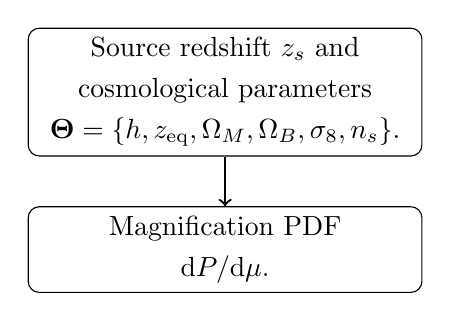
\begin{tikzpicture}[node distance=2.0cm]
\node[draw, rounded corners, align=center, minimum width=5.0cm] (input) 
{Source redshift $z_s$ and \\[1mm]
cosmological parameters \\[1mm]
$\vect{\Theta} = \{h,z_{\rm eq},\Omega_M,\Omega_B,\sigma_8,n_s\}$.};
\node[draw, rounded corners, align=center, minimum width=5.0cm, below of=input] (output)
{Magnification PDF \\[1mm]
$\mathrm{d}P/\mathrm{d}\mu$.};
\draw[->, thick] (input) -- (output);
\end{tikzpicture}
\end{center}

The emulator is a conditional normalizing flow that models the smooth body of the distribution, combined with a power-law tail calibrated to the $\mu^{-2}$ asymptote of Sec.~\ref{sec:pdf}, a fitted low-magnification edge, and a flux-conservation calibration that enforces $\langle\mu^{-1}\rangle=1$ on the emulated distribution. Each component is trained on Monte Carlo realizations of the extended lens model, sampled over a wide prior on $\vect\Theta$ and $z_s$. The resulting emulator reproduces held-out simulations with a median Kullback-Leibler divergence of $0.0073$\Gala{old result, I will update this once we train on the new subhalo design training will be done}, comparable to the value $0.007$ reported for ACE-Lensing~\cite{Turker:2025rdt}.
\Gala{i can also add some fancy ML related plots like ACE paper does}

\begin{figure}
    \centering
    
\includegraphics[width=1.0\columnwidth]{plots/variance_D_L.pdf}
    \caption{The variance of luminosity distances induced by weak lensing.}
    \label{fig:variance_DL}
\end{figure}


\subsection{Neural Spline Flow Architecture}

To capture the non-Gaussian shape of $dP_I/d\ln\mu$ with high accuracy across parameter space, we employ a Conditional Neural Spline Flow (NSF)~\cite{Durkan:2019nsq}. The flow models the target variable $x = \ln\mu$ conditioned on the context vector $\vect{c} = (z_s, \vect\Theta)$ through a sequence of $K = 6$ stacked monotonic rational-quadratic spline transformations. Each transformation divides the domain into $B = 8$ bins with linear extrapolation outside the standardized $[-3, 3]$ region. The bin widths, heights, and derivatives of the splines are generated by residual MLPs comprising 2 hidden layers with 128 hidden features per layer.
\begin{figure}
    \centering
    
\includegraphics[width=1.0\linewidth]{plots/fig_flow_transformation.pdf}
    \caption{Generative path of the conditional normalizing flow at $z_s = 5$ and the fiducial cosmology. The standardized Gaussian base density ($k=0$) is carried onto the magnification distribution $\td P_I/\td\mu$ by the $K=6$ stacked rational-quadratic spline transforms; each curve is the density of $2\times10^{6}$ samples after the $k$-th transform. The dashed curve is the flow density evaluated in closed form, which the final transform reproduces. The $\mu^{-2}$ tail, the empty-beam edge and the flux calibration are applied on top of this density and are not shown.}
    \label{fig:flow_transformation}
\end{figure}
Both the target variable $x = \ln\mu$ and context features $\vect{c}$ are standardized to zero mean and unit variance using pre-computed training set statistics, with exact log-Jacobian determinant corrections $-\ln\sigma_{\ln\mu}$ applied during probability density evaluations to maintain exact normalization. Figure~\ref{fig:flow_transformation} shows the density after each of the $K$ transforms, from the Gaussian base to the flow output.

\begin{figure}[t]
\centering
\def\NTRANS{3}      % transforms  (checkpoint: transforms=3)
\def\NBINS{10}      % spline bins (checkpoint: bins=10)
\begin{tikzpicture}[
    >={Stealth[length=1.8mm]},
    bus/.style={draw=black!55, line width=0.5pt},
    ar/.style={->, draw=black!55, line width=0.5pt},
    box/.style={rectangle, rounded corners=2.5pt, draw, align=center,
                inner sep=3.5pt, font=\scriptsize},
    lane/.style={box, text width=2.15cm, minimum height=1.95cm, anchor=north},
    neural/.style={lane, draw=blue!65!black, fill=blue!9},
    analytic/.style={lane, draw=orange!80!black, fill=orange!8, dashed},
    wide/.style={box, draw=black!65, fill=black!5, text width=7.4cm},
    tag/.style={font=\tiny, text=black!55, inner sep=1pt}
]

% ---- context -------------------------------------------------------------
\node[wide] (in) at (0,0)
  {source redshift and cosmology\\[0.6mm]
   $\vect{c} = \big(z_s,\,\vect\Theta\big), \quad
    \vect\Theta = \{h,\Omega_M,\Omega_B,\sigma_8,n_s,z_{\rm eq}\}$};

% ---- fan-out -------------------------------------------------------------
\draw[bus] (in.south) -- (0,-1.10);
\draw[bus] (-2.75,-1.10) -- (2.75,-1.10);
\draw[ar] (-2.75,-1.10) -- (-2.75,-1.45);
\draw[ar] (     0,-1.10) -- (     0,-1.45);
\draw[ar] ( 2.75,-1.10) -- ( 2.75,-1.45);

% ---- the three branches --------------------------------------------------
\node[neural]   (body) at (-2.75,-1.45)
  {conditioner MLP\\ $2\times128$\\[0.7mm]
   \NTRANS\ stacked\\ RQ splines\\ (\NBINS\ bins)\\[0.7mm]
   Student-$t$ base};
\node[analytic] (edge) at (0,-1.45)
  {demagnification\\ edge\\[0.7mm]
   $\mu_{\rm min}(\vect{c})$\\[0.7mm]
   fitted to the\\ simulations};
\node[analytic] (tail) at (2.75,-1.45)
  {fold-caustic tail\\[0.7mm]
   $\propto\mu^{-2}$\\[0.7mm]
   amplitude\\ regressed\\ on $\vect{c}$};

% ---- fan-in --------------------------------------------------------------
\draw[bus] (-2.75,-3.40) -- (-2.75,-4.00);
\draw[bus] (     0,-3.40) -- (     0,-4.00);
\draw[bus] ( 2.75,-3.40) -- ( 2.75,-4.00);
\draw[bus] (-2.75,-4.00) -- (2.75,-4.00);
\node[tag, anchor=west] at (-2.65,-3.68) {$p_{\rm body}$};
\node[tag, anchor=west] at ( 0.10,-3.68) {$\mu_{\rm min}$};
\node[tag, anchor=east] at ( 2.65,-3.68) {$p_{\rm tail}$};

% ---- combination ---------------------------------------------------------
\node[wide, anchor=north] (comb) at (0,-4.35)
  {blend body and tail at $\mu_c = 1.7$, truncate below $\mu_{\rm min}$,\\[0.5mm]
   renormalize, and shift to enforce $\langle\mu^{-1}\rangle = 1$};
\draw[ar] (0,-4.00) -- (0,-4.35);

% ---- output --------------------------------------------------------------
\node[box, draw=black!65, fill=black!5, text width=4.0cm, anchor=north]
      (out) at (0,-5.75)
  {$\mathrm{d}P_I/\mathrm{d}\ln\mu\,(z_s,\vect\Theta)$};
\draw[ar] (comb.south) -- (out.north);

% ---- legend --------------------------------------------------------------
\draw[draw=blue!65!black, fill=blue!9, rounded corners=1pt]
      (-3.10,-6.62) rectangle (-2.74,-6.42);
\node[tag, anchor=west] at (-2.66,-6.52) {learned};
\draw[draw=orange!80!black, fill=orange!8, dashed, rounded corners=1pt]
      (-1.20,-6.62) rectangle (-0.84,-6.42);
\node[tag, anchor=west] at (-0.76,-6.52)
      {analytic form, calibrated to the simulations};

\end{tikzpicture}
\caption{Structure of the emulator. The source redshift and the six cosmological parameters enter three branches. A conditioner network maps them onto the knots of \NTRANS\ stacked monotonic rational-quadratic spline transforms, which carry a Student-$t$ base density onto the body of $\mathrm{d}P_I/\mathrm{d}\ln\mu$. The other two branches set the demagnification edge and the amplitude of the $\mu^{-2}$ tail, whose shapes follow from Sec.~\ref{sec:pdf} and are not learned. The three combine into one normalized density obeying the flux sum rule.}
\label{fig:emulator_arch}
\end{figure}

\subsection{Composite PDF \& Tail Calibration}

The flow reproduces the body of the distribution but not its two ends. A finite number of spline bins cannot hold a sharp boundary, and the likelihood loss weights the rare high-magnification sightlines too weakly to fix the asymptotic slope. We therefore learn the body and impose both ends from Sec.~\ref{sec:pdf}.

The low-magnification edge enters as a window that suppresses the density below a demagnification bound $\mu_{\rm min}(z_s,\vect\Theta)$. We fit the bound to the $0.1\%$ quantile of the simulated distributions and keep the window smooth rather than truncating, because the simulator retains a small population of strongly demagnified sightlines below it.

The high-magnification tail enters as a power law approaching the $\mu^{-2}$ asymptote of Sec.~\ref{sec:pdf}. We set its amplitude by regressing the exceedance probabilities at $\mu = 2$, $3$ and $8$ on the context, and we join it to the body with a smooth blend at $\mu_c = 1.7$ rather than splicing them, so the composite density carries no kink.

A final shift in $\ln\mu$ matches the mean inverse magnification of the emulated distribution to that of the simulated one, evaluated over the support on which both are defined. Figure~\ref{fig:emulator_arch} shows the three branches and their combination.

We train the flow by minimizing the negative log-likelihood on Monte Carlo realizations drawn over a Latin hypercube in $z_s$ and $\vect\Theta$, and we evaluate it on held-out configurations that enter neither the flow nor the edge and tail fits. The emulator reproduces the held-out simulations with a median Kullback-Leibler divergence of $0.0073$, comparable to the value $0.007$ reported for ACE-Lensing~\cite{Turker:2025rdt}. Imposing the edge and the flux calibration is what brings it there. Measured instead on a fixed fine binning across the validation panels, so that the two are read off the same ruler, they lower the median divergence from $0.0051$ to $0.0034$ and the mean from $0.0091$ to $0.0035$, and they remove the largest single-panel failures near $z_s = 1$.

\begin{figure}
    \centering
    
\includegraphics[width=1.0\columnwidth]{plots/variance_D_L.pdf}
    \caption{The variance of luminosity distances induced by weak lensing.The curves show, cumulatively, the lens model of Ref.~\cite{Vaskonen:2026ubd}, the effect of adding the subhalo population, and the effect of adding the correlated clustering of field halos. \Gala{add Takahashi i think and Mptetha}}
    \label{fig:variance_DL}
\end{figure}
Figure~\ref{fig:variance_DL} shows the resulting variance of the luminosity distance, $\sigma_{D_L}(z,\vect\Theta)$, and decomposes it into the contributions of the two ingredients introduced in this work, in the same way that Ref.~\cite{Vaskonen:2026ubd} separates the effects of halo ellipticity, bias and filaments. Both act on the width of the magnification distribution rather than on its position, and both raise the lensing scatter: subhalos by adding small-scale structure within each lens, and correlated clustering by making the discrete lens counts along a sightline fluctuate coherently. Neither is captured by scatter budgets built from smooth-halo calculations.



\section{Comparison with earlier works}
\label{sec:comparison}

\Gala{we can compare with the following:
\begin{enumerate}
    \item ACE-lensing
    \item halo/subhalo population comparison with pyhalo
    \item Mpetha 24
    \item ...
\end{enumerate}
}

\section{Conclusions}
\label{sec:conclusions}

\section*{Acknowledgments} 
This work was supported by the Estonian Research Council grants TARISTU24-TK3 and TARISTU24-TK10, and the Center of Excellence program TK202 of the Estonian Ministry of Education and Research.

\bibliography{refs}

\end{document}
